\documentclass[12pt]{article}

% -------------------------
% PAQUETES NECESARIOS
% -------------------------
\usepackage[utf8]{inputenc}
\usepackage[T1]{fontenc}
\usepackage{titlesec}
\usepackage{fancyhdr}
\usepackage{graphicx}
\usepackage{listings}
\usepackage{xcolor}
\usepackage{geometry}
\usepackage[spanish]{babel}
\usepackage{graphicx}
\usepackage{booktabs} % Para líneas profesionales (\toprule, \midrule, \bottomrule)
\usepackage{multirow} % Para agrupar celdas verticales

\usepackage{amsmath}
\usepackage{booktabs}
\usepackage{xcolor}
\usepackage{pgfplots}
\pgfplotsset{compat=1.18}
\usepackage[colorlinks=true, linkcolor=blue, citecolor=blue, urlcolor=blue]{hyperref}


\usepackage{algorithm}
\usepackage{algpseudocode}
\floatname{algorithm}{Algoritmo}
\algrenewcommand\algorithmicif{\textbf{si}}
\algrenewcommand\algorithmicthen{\textbf{entonces}}
\algrenewcommand\algorithmicelse{\textbf{si no}}
\algrenewcommand\algorithmicend{\textbf{fin}}
\algrenewcommand\algorithmicfor{\textbf{para}}
\algrenewcommand\algorithmicdo{\textbf{hacer}}
\algrenewcommand\algorithmicwhile{\textbf{mientras}}
\algrenewcommand\algorithmicfunction{\textbf{función}}
\algrenewcommand\algorithmicreturn{\textbf{devolver}}
\algrenewtext{EndIf}{\textbf{fin si}}
\algrenewtext{EndFor}{\textbf{fin para}}
\algrenewtext{EndWhile}{\textbf{fin mientras}}
\algrenewtext{EndFunction}{\textbf{fin función}}



% Definición de colores principales
\definecolor{primary}{RGB}{30, 64, 175}
\definecolor{secondary}{RGB}{13, 148, 136}
\definecolor{danger}{RGB}{225, 29, 72}
\definecolor{neutral-bg}{RGB}{248, 250, 252}


% -------------------------
% CONFIGURACIÓN DE PÁGINA
% -------------------------
\geometry{margin=2.5cm}

% Fuente tipo Times New Roman equivalente
\usepackage{mathptmx}

% Interlineado sencillo (por defecto en LaTeX)

% -------------------------
% CONFIGURACIÓN DE ENCABEZADO Y PIE
% -------------------------
\pagestyle{fancy}
\setlength{\headheight}{15pt}
\setlength{\emergencystretch}{2em}
\fancyhf{}

\fancyhead[L]{Metodología de la programación paralela}
\fancyhead[R]{2026/2027}

\fancyfoot[L]{Andrey, Abdellah} % <-- EDITAR
\fancyfoot[R]{\thepage}

\renewcommand{\headrulewidth}{0.4pt}
\renewcommand{\footrulewidth}{0.4pt}


\usepackage{listings}
\usepackage{xcolor}

% --- Colores generales ---
\definecolor{mGreen}{rgb}{0,0.6,0}
\definecolor{mGray}{rgb}{0.5,0.5,0.5}
\definecolor{mPurple}{rgb}{0.58,0,0.82}
\definecolor{bgC}{rgb}{0.98,0.98,0.98}
\definecolor{bgValgrind}{rgb}{0.93,0.93,0.93}

% --- ESTILO 1: Para Código C ---
\lstdefinestyle{EstiloC}{
    backgroundcolor=\color{bgC},
    commentstyle=\color{mGreen}\itshape,
    keywordstyle=\color{magenta}\bfseries,
    numberstyle=\tiny\color{mGray},
    stringstyle=\color{mPurple},
    basicstyle=\ttfamily\footnotesize,
    breakatwhitespace=false,
    breaklines=true,                 % ¡Evita que el código se salga por la derecha!
    captionpos=b,
    keepspaces=true,
    numbers=left,
    numbersep=8pt,
    showstringspaces=false,
    tabsize=4,
    language=C,
    frame=single,
    rulecolor=\color{mGray!30}
}

% --- ESTILO 2: Para trazas/logs de Valgrind ---
\lstdefinestyle{EstiloValgrind}{
    backgroundcolor=\color{bgValgrind},
    basicstyle=\ttfamily\scriptsize, % Letra ligeramente más pequeña para trazas anchas
    breakatwhitespace=false,
    breaklines=true,                 % ¡Evita que los reportes de Valgrind se corten!
    captionpos=b,
    frame=single,
    numbers=none,                    % Sin números de línea para logs de terminal
    showstringspaces=false,
    language={},                     % Sin resaltado de sintaxis de lenguaje
    rulecolor=\color{mGray!50}
}

% -------------------------
% INICIO DEL DOCUMENTO
% -------------------------
% acentos y eñes dentro de los listados de código (sin esto, listings falla con UTF-8)
\lstset{literate=
  {á}{{\'a}}1 {é}{{\'e}}1 {í}{{\'i}}1 {ó}{{\'o}}1 {ú}{{\'u}}1
  {Á}{{\'A}}1 {É}{{\'E}}1 {Í}{{\'I}}1 {Ó}{{\'O}}1 {Ú}{{\'U}}1
  {ñ}{{\~n}}1 {Ñ}{{\~N}}1 {ü}{{\"u}}1}

\begin{document}

% =========================
% PORTADA
% =========================
\thispagestyle{empty}

% Bloque arriba a la derecha
\begin{flushright}
Abdellah Bensaidi, Souri 1.3\\
Morales Vicuña, Andrey 1.1\\
Asignatura: Metodología de la programación paralela \\
Grupo: 1 \\
Práctica 3: Paralelización híbrida con MPI+OpenMP. Modelado y auto-optimización \\
\end{flushright}

\vfill

\begin{center}

\includegraphics[width=0.4\textwidth]{sello.png}
\end{center}

\vfill

\begin{center}
\today
\end{center}

\newpage
\tableofcontents
\newpage

% =========================
% SISTEMA COMPUTACIONAL
% =========================
\section{Sistema computacional}

% >>> DATO: generar en el ordenador de las ejecuciones finales con
%   lstopo -f -p --no-legend --no-io sistema.svg
% y convertirlo para LaTeX con:  rsvg-convert -f pdf -o sistema.pdf sistema.svg
% (o directamente: lstopo -f -p --no-legend --no-io sistema.pdf)
\begin{figure}[htbp]
    \centering
    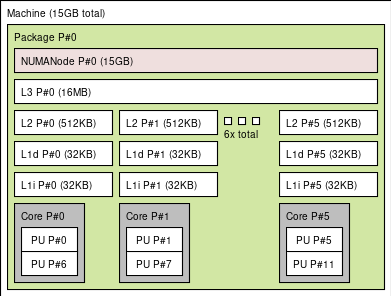
\includegraphics[width=0.8\textwidth]{sistema.png}
    \caption{Sistema utilizado (salida de \texttt{lstopo -f -p -{}-no-legend -{}-no-io}).}
    \label{fig:sistema}
\end{figure}

% >>> DATO: descripción de la máquina de las ejecuciones finales
Todas las ejecuciones se han realizado en el mismo sistema: un procesador AMD Ryzen 5 5500 con 6 núcleos físicos y 12 hilos hardware (2 hilos por núcleo mediante SMT) en un único socket. Dispone de caché L1d de 32 KiB y L1i de 32 KiB por núcleo, L2 de 512 KiB por núcleo y L3 de 16 MiB compartida, y aproximadamente 15,8 GB de memoria RAM. La frecuencia máxima es de 4,46 GHz. Se ha usado Ubuntu 24.04, \texttt{gcc} con \texttt{-O3} y OpenMPI.

\newpage

\section{Ejercicios}

\begin{enumerate}

% =====================================================================
%  PARTE 1
% =====================================================================
\item[] \textbf{\large Parte 1. Implementación de paralelismo híbrido (MPI + OpenMP)}

\item \textbf{Cuestión 1.} Con el fin de obtener un código más eficiente en la parte de memoria compartida y poder maximizar el proceso de mejora de la población de individuos: reemplazar las llamadas a la función \texttt{rand} por \texttt{rand\_r} (que es ``thread safe'') para evitar, por un lado, que se genere la misma secuencia de valores aleatorios en diferentes hilos y, por otro, que se pierda paralelismo durante la generación de dichos valores debido a la secuencialidad que introduce la función \texttt{rand}.

% --- Respuesta de la cuestión 1 ---

Se parte del código de la cuestión 6 de la P2 (modelo de islas con comunicaciones colectivas), que es el que se usará en la versión híbrida. Todos los números aleatorios del algoritmo se obtienen con la función \texttt{aleatorio}, así que basta con cambiarla a ella y a la inicialización de la semilla.

\medskip
\noindent\textbf{Generación de números aleatorios (\texttt{mh.c})}\par
\smallskip

\begin{lstlisting}[style=EstiloC]
// rand_r recibe el estado (la semilla) como parámetro, así que es "thread safe", y con
// threadprivate cada hilo tiene su propia copia de la semilla
static unsigned int semilla = 1;
#pragma omp threadprivate(semilla)

int aleatorio(int n) {
	return (rand_r(&semilla) % n);  // genera un numero aleatorio entre 0 y n-1
}
\end{lstlisting}

\textbf{Justificación:} \texttt{rand} guarda su estado en una variable global que comparten todos los hilos. En bibliotecas que protegen ese estado compartido, las llamadas concurrentes pueden serializarse. Un estado separado por hilo evita esa contención; semillas distintas no garantizan por sí solas independencia estadística. \texttt{rand\_r} recibe el estado como parámetro, y con \texttt{threadprivate} cada hilo tiene su propia semilla, de modo que no se comparte nada y cada hilo genera su propia secuencia. Se ha hecho igual que en la P1.

\vspace{0.5cm}

\medskip
\noindent\textbf{Inicialización de la semilla (\texttt{aplicar\_mh} en \texttt{mh.c})}\par
\smallskip

\begin{lstlisting}[style=EstiloC]
// P3 CUESTIÓN 1: en lugar de srand se inicializa la semilla de rand_r
semilla = (unsigned int) (time(NULL) + getpid() + rank * 1000);
\end{lstlisting}

\textbf{Justificación:} Sustituye al \texttt{srand} de la P2. Se mantiene el \texttt{rank} para que cada isla tenga una semilla distinta y evolucione de forma diferente. En esta cuestión todavía no hay hilos, así que hay una semilla por proceso; en la cuestión 2 se añade el número de hilo para que cada hilo de cada proceso tenga la suya. En el \texttt{Makefile} se ha añadido \texttt{-fopenmp} para que se reconozca la directiva \texttt{threadprivate}. La corrección se ha comprobado verificando los genes de las soluciones y recalculando su fitness. Cambiar el generador puede cambiar la secuencia aleatoria y el fitness final respecto a P2.


\newpage
\item \textbf{Cuestión 2.} Implementar un algoritmo híbrido, tomando como referencia las directivas OpenMP y primitivas MPI que arrojaron mejores resultados en las prácticas 1 y 2. Se deberán utilizar, por tanto, las funciones que se considere más adecuadas para obtener un código optimizado y que permita obtener las mejores prestaciones. Ejecutar el código variando el número de procesos y de hilos, y comparar los resultados obtenidos respecto a la versión secuencial utilizando las métricas de rendimiento de la Tabla 1.

Además, se deberá analizar la mejora obtenida en las prestaciones, considerando solo tiempo de ejecución y tiempo de ejecución + fitness (ver apartado (1) de Observaciones), respecto al algoritmo secuencial y también respecto a la mejor versión paralela obtenida en las prácticas anteriores usando el mismo sistema computacional para todas las versiones.

% --- Respuesta de la cuestión 2 ---

La versión híbrida combina las dos mejores versiones de las prácticas anteriores:

\begin{itemize}
    \item \textbf{Nivel MPI (P2, cuestión 6):} modelo de islas con comunicaciones colectivas. Cada proceso es una isla y cada NGM generaciones el proceso 0 recoge los NEM mejores de cada isla con \texttt{MPI\_Gather} y les devuelve los NEM mejores globales y la decisión de parar con \texttt{MPI\_Bcast}.
    \item \textbf{Nivel OpenMP (P1):} dentro de cada proceso, una única región paralela para todo el algoritmo, con los bucles sobre la población repartidos entre los hilos.
\end{itemize}

A continuación se muestran las partes del código modificadas respecto a la cuestión 1.

% cambio 1: inicialización de MPI con hilos

\medskip
\noindent\textbf{Inicialización de MPI y número de hilos (\texttt{main.c})}\par
\smallskip

\begin{lstlisting}[style=EstiloC]
int provided;
MPI_Init_thread(&argc, &argv, MPI_THREAD_FUNNELED, &provided);
...
if (provided < MPI_THREAD_FUNNELED) {
	...
	MPI_Finalize();
	return EXIT_FAILURE;
}
...
int NHILOS = atoi(argv[8]); // P3: hilos OpenMP que pone en marcha cada proceso
assert(NHILOS >= 1);
omp_set_num_threads(NHILOS);
\end{lstlisting}

\textbf{Justificación:} Cuando un proceso MPI tiene varios hilos hay que avisar a MPI de cómo se van a usar con \texttt{MPI\_Init\_thread}. Se pide el nivel \texttt{MPI\_THREAD\_FUNNELED}, que significa que solo el hilo maestro hace llamadas a MPI. Es el nivel más bajo que nos sirve, porque en nuestro código todas las comunicaciones las hace el maestro (ver más abajo), y los niveles más altos añaden cerrojos dentro de MPI que no necesitamos. Si la biblioteca no lo soporta, el programa termina. El número de hilos por proceso se pasa como un nuevo argumento para poder probar combinaciones de procesos e hilos sin recompilar.

\vspace{0.5cm}

% cambio 2: región paralela

\medskip
\noindent\textbf{Algoritmo híbrido (\texttt{aplicar\_mh} en \texttt{mh.c})}\par
\smallskip

\begin{lstlisting}[style=EstiloC]
MPI_Comm comm = MPI_COMM_WORLD;
MPI_Datatype mpi_int = MPI_INT;

#pragma omp parallel default(none) \
	shared(d, n, m, n_gen, tam_pob, m_rate, sol, NGM, NEM, rank, size, individuo_type, comm, mpi_int, \
	       tam_local, bloque, poblacion, emigrantes, inmigrantes, mezcla, p_mezcla, \
	       fitness_modelo, ngeneracion, continuar, value)
{
	// P3 CUESTIÓN 1: semilla distinta para cada hilo de cada proceso
	int id = 0;
#if defined (_OPENMP)
	id = omp_get_thread_num();
#endif
	semilla = (unsigned int) (time(NULL) + getpid() + rank * 1000 + 7919 * id);

	#pragma omp for schedule(dynamic)
	for (int i = 0; i < tam_local; i++) {
		poblacion[i] = &bloque[i];
		crear_individuo(n, m, poblacion[i]->array_int);
		fitness(d, poblacion[i], n, m);
	}

	#pragma omp single
	{
		qsort(poblacion, tam_local, sizeof(Individuo *), comp_fitness);
		fitness_modelo = poblacion[0]->fitness;
	}

	int g = 0;
	while (g < n_gen && continuar)
	{
		int gen_bloque = 0;
		for (int k = 0; k < NGM && g < n_gen; k++, g++, gen_bloque++)
		{
			#pragma omp for schedule(dynamic)
			for (int i = 0; i < (tam_local/2) - 1; i += 2) {
				cruzar(poblacion[i], poblacion[i+1], poblacion[tam_local/2 + i], poblacion[tam_local/2 + i + 1], n, m);
			}

			#pragma omp for schedule(static)
			for (int i = 0; i < tam_local; i++) {
				if (i >= tam_local/4)
					mutar(poblacion[i], n, m, m_rate);
				fitness(d, poblacion[i], n, m);
			}

			#pragma omp single
			qsort(poblacion, tam_local, sizeof(Individuo *), comp_fitness);
		}

		// Migración: solo el hilo maestro de cada proceso llama a MPI
		#pragma omp master
		{
			copiar_mejores(poblacion, emigrantes, NEM);
			MPI_Gather(emigrantes, NEM, individuo_type, mezcla, NEM, individuo_type, 0, comm);
			if (rank == 0) {
				... // ordenar la mezcla, elegir los NEM mejores y decidir la convergencia
			}
			MPI_Bcast(inmigrantes, NEM, individuo_type, 0, comm);
			MPI_Bcast(&continuar, 1, mpi_int, 0, comm);
			reemplazar_peores(poblacion, tam_local, inmigrantes, NEM);
		}
		#pragma omp barrier
	}

	// Resultado final: el proceso 0 recoge el mejor de cada isla (solo el maestro)
	#pragma omp master
	{
		... // MPI_Gather del mejor de cada isla y copia del mejor global en sol
	}
} // fin de la región paralela (barrera implícita)
\end{lstlisting}

\textbf{Justificación:}

\begin{itemize}
    \item \textbf{Una sola región paralela.} Como en la P1, los hilos se crean una vez al principio y no en cada generación, para no pagar el coste de crearlos muchas veces. Con \texttt{default(none)} estamos obligados a indicar el alcance de cada variable, lo que evita compartir algo sin querer. En OpenMPI, \texttt{MPI\_COMM\_WORLD} y \texttt{MPI\_INT} son variables globales y \texttt{default(none)} da error con ellas, por eso se copian a las variables locales \texttt{comm} y \texttt{mpi\_int}.
    \item \textbf{Semilla por hilo.} A la semilla de la cuestión 1 se le suma el número de hilo multiplicado por un primo, para que cada hilo de cada proceso genere una secuencia distinta.
    \item \textbf{Reparto de los bucles.} Se usan las mismas directivas que dieron mejor resultado en la P1. La población inicial y el cruce usan \texttt{schedule(dynamic)} porque cada iteración tiene un coste distinto (crear un individuo y reparar los duplicados del cruce tardan más o menos según los números que salgan). La mutación y el fitness se han juntado en un solo bucle, porque el fitness de un individuo solo depende de su propia mutación; así hay una barrera menos por generación. Este bucle usa \texttt{schedule(static)}, porque su coste lo marca el fitness, que es igual para todos los individuos. La ordenación con \texttt{qsort} es secuencial y la hace un solo hilo con \texttt{single}. La barrera implícita de cada \texttt{for} es necesaria: la mutación modifica individuos que son padres en el cruce, y no se puede ordenar hasta que todos tengan su fitness.
    \item \textbf{Comunicaciones solo en el hilo maestro.} La migración y la recogida final del resultado van dentro de \texttt{master}, que es lo que permite usar el nivel \texttt{FUNNELED}. Como \texttt{master} no tiene barrera implícita, se pone un \texttt{barrier} después: ningún hilo puede seguir con la población ni leer \texttt{continuar} hasta que el maestro haya terminado la migración. Así todos los hilos de todos los procesos salen del bucle en la misma generación y no hay bloqueos.
    \item \textbf{Variables privadas y compartidas.} El contador de generaciones \texttt{g} es privado, pero todos los hilos hacen las mismas iteraciones, así que vale lo mismo en todos. \texttt{continuar} es compartida: la escribe el maestro y el resto la lee después de la barrera.
\end{itemize}

Se ha comprobado que la solución es correcta volviendo a calcular su fitness a partir de la matriz de distancias. También se ha comprobado que no hay bloqueos con distintas combinaciones de procesos e hilos y con migración en cada generación (NGM = 1).

\vspace{0.5cm}

\medskip
\noindent\textbf{Compilación y ejecución}\par
\smallskip

En el \texttt{Makefile} se ha añadido \texttt{-fopenmp} y el número de hilos como parámetro, y se ejecuta con \texttt{mpirun -{}-bind-to none}. Una afinidad demasiado restrictiva impuesta por el lanzador puede limitar los hilos de cada proceso. Con \texttt{-{}-bind-to none} se desactiva esa afinidad y el sistema operativo puede distribuirlos entre los núcleos disponibles; los valores por defecto dependen de la configuración de MPI.

\vspace{0.5cm}

\medskip
\noindent\textbf{Experimentos}\par
\smallskip

Para comparar todas las versiones en el mismo sistema, como pide el enunciado, se han vuelto a ejecutar en la misma sesión y alternadas, con el script \texttt{experimentos\_c2.sh}:

\begin{itemize}
    \item \textbf{Secuencial:} el código de la P1 compilado sin OpenMP. Es el que se usa como tiempo secuencial para calcular el speed-up.
    \item \textbf{P1 (OpenMP):} la mejor versión de la P1 con 2, 4, 6 y 12 hilos.
    \item \textbf{P2 (MPI):} la versión elegida en la cuestión 6 de la P2 (colectivas) con 2, 4, 6 y 12 procesos.
    \item \textbf{Híbrida:} todas las combinaciones de procesos e hilos con EP = 1, 2, 4, 6 y 12 elementos de proceso (EP = n\_procesos $\cdot$ n\_hilos).
\end{itemize}

En la copia del código de la P1 se han corregido dos errores que ya se habían corregido en la P2 para que la comparación sea justa: la función de ordenación \texttt{comp\_fitness} devolvía como \texttt{int} la resta de dos \texttt{double}, y en \texttt{distancia\_ij} estaba comentado el intercambio de \texttt{i} y \texttt{j}.

% >>> DATO: instancia, NGM, NEM y repeticiones
Se ha usado la instancia \texttt{n = 2000, m = 800, n\_gen = 400, tam\_pob = 200, m\_rate = 0.3}, con NGM = 10 y NEM = 3 (los valores elegidos en la P2), y cada configuración se ha ejecutado 3 veces tomando la media. Como en la P2, cada versión se ha ejecutado de dos formas:

\begin{itemize}
    \item \textbf{Trabajo fijo:} siempre 60 generaciones, sin criterio de convergencia (compilando con \texttt{-DSIN\_CONVERGENCIA}). Se iguala el presupuesto de generaciones, evitando comparar tiempos de ejecuciones que paran tras un número distinto de ellas; el reparto en islas puede cambiar las transformaciones realizadas.
    \item \textbf{Con convergencia:} el algoritmo normal, que para cuando el fitness deja de mejorar. Con esta se compara tiempo y fitness con el indicador $I = \text{fitness}/\text{tiempo}$ de la observación 1.
\end{itemize}

% >>> DATO: tiempos de trabajo fijo del híbrido (resultados_c2/resumen.txt, filas "fijo hibrido")
\begin{table}[htbp]
\centering
\begin{tabular}{ccc|ccc}
\toprule
\textbf{n\_procesos} & \textbf{n\_hilos} & \textbf{EP} & \textbf{t\_ejec (s)} & \textbf{speed-up} & \textbf{eficiencia} \\
\midrule
1 & 1 & 1 & 13.737 & 1.04 & 1.04 \\
\midrule
1 & 2 & \multirow{2}{*}{2} & \textbf{6.893} & \textbf{2.08} & 1.04 \\
2 & 1 & & 11.238 & 1.27 & 0.64 \\
\midrule
1 & 4 & \multirow{3}{*}{4} & \textbf{3.700} & \textbf{3.87} & 0.97 \\
2 & 2 & & 6.140 & 2.33 & 0.58 \\
4 & 1 & & 8.119 & 1.76 & 0.44 \\
\midrule
1 & 6 & \multirow{4}{*}{6} & \textbf{2.616} & \textbf{5.47} & 0.91 \\
2 & 3 & & 4.904 & 2.92 & 0.49 \\
3 & 2 & & 5.552 & 2.58 & 0.43 \\
6 & 1 & & 6.949 & 2.06 & 0.34 \\
\midrule
1 & 12 & \multirow{6}{*}{12} & \textbf{2.223} & \textbf{6.44} & 0.54 \\
2 & 6 & & 4.316 & 3.31 & 0.28 \\
3 & 4 & & 5.337 & 2.68 & 0.22 \\
4 & 3 & & 6.228 & 2.30 & 0.19 \\
6 & 2 & & 6.590 & 2.17 & 0.18 \\
12 & 1 & & 7.880 & 1.82 & 0.15 \\
\bottomrule
\end{tabular}
\caption{Prestaciones de la versión híbrida con trabajo fijo (\texttt{n = 2000, m = 800, n\_gen = 60, tam\_pob = 200, m\_rate = 0.3}, NGM = 10, NEM = 3). El speed-up se calcula respecto al secuencial (14.307 s) y la eficiencia es speed-up/EP. En negrita, la mejor configuración para cada EP.}
\label{tab:c2_hibrido}
\end{table}

% >>> DATO: comparación de versiones (filas "fijo" y "convergencia" de resultados_c2/resumen.txt).
% Para el híbrido se pone la mejor configuración de cada EP.
\begin{table}[htbp]
\centering
\small
\begin{tabular}{lcc|cc|ccc}
\toprule
 & & & \multicolumn{2}{c|}{\textbf{Trabajo fijo}} & \multicolumn{3}{c}{\textbf{Con convergencia}} \\
\textbf{Versión} & \textbf{p $\times$ h} & \textbf{EP} & \textbf{t (s)} & \textbf{speed-up} & \textbf{t (s)} & \textbf{fitness} & \textbf{I ($\cdot 10^6$)} \\
\midrule
Secuencial & 1 $\times$ 1 & 1 & 14.307 & 1.00 & 3.860 & 16\,051\,808 & 4.16 \\
\midrule
P1 (OpenMP) & 1 $\times$ 2 & 2 & 6.794 & 2.11 & 1.838 & 16\,045\,310 & 8.73 \\
P2 (MPI) & 2 $\times$ 1 & 2 & 11.439 & 1.25 & 4.010 & 16\,047\,989 & 4.00 \\
Híbrida & 1 $\times$ 2 & 2 & 6.893 & 2.08 & 2.387 & 16\,052\,357 & 6.72 \\
\midrule
P1 (OpenMP) & 1 $\times$ 4 & 4 & 3.587 & 3.99 & 0.978 & 16\,046\,713 & 16.41 \\
P2 (MPI) & 4 $\times$ 1 & 4 & 8.162 & 1.75 & 2.853 & 16\,046\,052 & 5.62 \\
Híbrida & 1 $\times$ 4 & 4 & 3.700 & 3.87 & 1.276 & 16\,045\,683 & 12.58 \\
\midrule
P1 (OpenMP) & 1 $\times$ 6 & 6 & 2.605 & 5.49 & 0.697 & 16\,045\,589 & 23.02 \\
P2 (MPI) & 6 $\times$ 1 & 6 & 6.964 & 2.05 & 2.396 & 16\,057\,280 & 6.70 \\
Híbrida & 1 $\times$ 6 & 6 & 2.616 & 5.47 & 0.906 & 16\,045\,713 & 17.72 \\
\midrule
P1 (OpenMP) & 1 $\times$ 12 & 12 & 2.215 & 6.46 & 0.587 & 16\,043\,639 & 27.32 \\
P2 (MPI) & 12 $\times$ 1 & 12 & 7.854 & 1.82 & 2.700 & 16\,052\,091 & 5.95 \\
Híbrida & 1 $\times$ 12 & 12 & 2.223 & 6.44 & 0.754 & 16\,047\,076 & 21.28 \\
\bottomrule
\end{tabular}
\caption{Comparación local de las versiones secuencial, OpenMP, MPI e híbrida: n=2000, m=800, tam\_pob=200 y m\_rate=0.3; NGM=10 y NEM=3 en las versiones con islas. Cada columna usa la media de tres ejecuciones del modo correspondiente: 60 generaciones en trabajo fijo y un máximo de 400 con convergencia. La referencia secuencial del speed-up de trabajo fijo es 14.307 s. $I=\overline{fitness}/\overline{tiempo}$.}
\label{tab:c2_comparacion}
\end{table}

% >>> DATO: los mismos tiempos de trabajo fijo de las tablas anteriores
\begin{figure}[htbp]
\centering
\begin{tikzpicture}
\begin{axis}[
    width=0.48\textwidth, height=6cm,
    xlabel={EP (procesos $\cdot$ hilos)}, ylabel={Tiempo (s)},
    xtick={1,2,4,6,12}, ymin=0,
    legend style={font=\footnotesize, at={(0.98,0.98)}, anchor=north east},
    grid=major, title={\small Tiempo con trabajo fijo}]
\addplot[mark=*, blue] coordinates {(1,14.307) (2,6.794) (4,3.587) (6,2.605) (12,2.215)};
\addlegendentry{P1 (OpenMP)}
\addplot[mark=square*, red] coordinates {(1,14.307) (2,11.439) (4,8.162) (6,6.964) (12,7.854)};
\addlegendentry{P2 (MPI)}
\addplot[mark=triangle*, teal] coordinates {(1,13.737) (2,6.893) (4,3.700) (6,2.616) (12,2.223)};
\addlegendentry{Híbrida 1 $\times$ h}
\end{axis}
\end{tikzpicture}
\hfill
\begin{tikzpicture}
\begin{axis}[
    width=0.48\textwidth, height=6cm,
    xlabel={n\_procesos (n\_hilos = 12/n\_procesos)}, ylabel={Tiempo (s)},
    xtick={1,2,3,4,6,12}, ymin=0,
    grid=major, title={\small Híbrida con EP = 12}]
\addplot[mark=triangle*, teal] coordinates {(1,2.223) (2,4.316) (3,5.337) (4,6.228) (6,6.590) (12,7.880)};
\end{axis}
\end{tikzpicture}
\caption{Izquierda: tiempo con trabajo fijo de cada versión al aumentar los elementos de proceso. Derecha: tiempo de la versión híbrida con 12 elementos de proceso repartidos de distintas formas entre procesos e hilos.}
\label{fig:c2}
\end{figure}

\medskip
\noindent\textbf{Análisis}\par
\smallskip

% >>> DATO: revisar los números citados si cambian las tablas
\begin{itemize}
    \item \textbf{Reparto entre procesos e hilos.} Para cada EP probado, el menor tiempo híbrido se obtiene con un proceso. Con EP=12 se pasa de 2.223 s con $1\times12$ a 7.880 s con $12\times1$. Cada proceso mantiene una copia de la matriz, mientras que sus hilos la comparten. Las comunicaciones, las esperas, el tamaño de las islas y la competencia por memoria y caché son factores plausibles; los tiempos totales no permiten atribuir por separado su contribución.
    \item \textbf{Respecto al secuencial.} La configuración híbrida $1\times12$ obtiene un speed-up de 6.44 y una eficiencia de 0.54. Doce hilos hardware comparten los recursos de seis núcleos físicos mediante SMT. Con $1\times1$, el tiempo es 13.737 s frente a 14.307 s secuencial; diferencias de trayectoria aleatoria y variación de las medidas pueden intervenir. Una eficiencia mayor que uno no es una medida directa de ocupación de CPU.
    \item \textbf{Respecto a OpenMP.} Con trabajo fijo y doce hilos, P1 tarda 2.215 s y el híbrido $1\times12$, 2.223 s: una diferencia de unos 0.008 s, pequeña frente a la variación de las repeticiones. Con una isla, el híbrido conserva las comunicaciones y copia los mejores sobre los peores; por tanto, su evolución no es exactamente la del secuencial o P1.
    \item \textbf{Respecto a MPI.} A igual EP=12, P2 tarda 7.854 s y el híbrido 2.223 s, una razón aproximada de 3.53. La mejor configuración MPI de todas las medidas es la de seis procesos: 6.964 s, speed-up 2.05. Respecto a esa mejor configuración global, el híbrido es unas 3.13 veces más rápido. No se debe confundir la comparación a igual EP con la comparación entre los mejores resultados de cada familia.
    \item \textbf{Tiempo y fitness.} Las medias de fitness de las configuraciones están próximas, por lo que el indicador $I$ queda dominado en gran medida por el tiempo. Con convergencia, el híbrido $1\times12$ obtiene $I=21.28\cdot10^6$, frente a $4.16\cdot10^6$ del secuencial, $6.70\cdot10^6$ de la mejor configuración MPI (seis procesos) y $27.32\cdot10^6$ de OpenMP con doce hilos. Se trata de razones aproximadas de 5.12 y 3.18 respecto al secuencial y a la mejor MPI, respectivamente.
    \item \textbf{Criterios de parada.} P1 comprueba la mejora cada generación y el híbrido en los bloques de NGM=10. Con convergencia pueden hacer distintas cantidades de trabajo antes de parar. La comparación con 60 generaciones fijas iguala el presupuesto de generaciones, aunque el reparto en islas y sus migraciones no reproducen exactamente una misma trayectoria evolutiva.
\end{itemize}

Para esta instancia y las configuraciones medidas, el mejor híbrido es $1\times12$: alrededor de 6.44 veces más rápido que el secuencial y 3.13 veces más rápido que la mejor configuración MPI, con un tiempo muy próximo al de OpenMP con doce hilos.


% =====================================================================
%  PARTE 2
% =====================================================================
\newpage
\item[] \textbf{\large Parte 2. Modelado y auto-optimización del algoritmo paralelo}

En la parte 2 se utiliza el fichero \texttt{io.c} del material de ejecución proporcionado. Este genera la matriz de distancias directamente en memoria, sin leer ficheros de entrada.

\item \textbf{Cuestión 3.} Modelo de tiempo en memoria compartida con un nivel de paralelismo.

% =====================================================================
% CUESTIÓN 3: sustituir todo lo que hay debajo de la línea
%   % --- Respuesta de la cuestión 3 ---
% hasta el \newpage de la cuestión 4 por este texto.
% Los datos están marcados con "% >>> DATO" (no salen en el PDF).
% =====================================================================

Esta cuestión parte del código de la P1 (OpenMP), con los dos errores corregidos en la cuestión 2, y con el nuevo \texttt{io.c}, que genera la matriz de distancias en memoria. A continuación se muestran las partes del código modificadas.

\medskip
\noindent\textbf{3.1 Obtención de datos experimentales}\par
\smallskip

% cambio 1: parámetros

\medskip
\noindent\textbf{Nuevos parámetros N\_HILOS\_INI y N\_HILOS\_FIT (\texttt{main.c})}\par
\smallskip

\begin{lstlisting}[style=EstiloC]
if(argc < 7) {
	fprintf(stderr,"Ayuda:\n");
	fprintf(stderr,"  ./programa n m nGen tamPob N_HILOS_INI N_HILOS_FIT [m_rate]\n");
	return(EXIT_FAILURE);
}
...
int n_hilos_ini = atoi(argv[5]);   // hilos del bucle de la población inicial (FOR_INI)
int n_hilos_fit = atoi(argv[6]);   // hilos del bucle del fitness (FOR_FIT)
// m_rate pasa a ser opcional (por defecto 0.3) porque el Makefile del profesor no lo pasa
double m_rate = (argc > 7) ? atof(argv[7]) : 0.3;
assert(n_hilos_ini >= 1 && n_hilos_fit >= 1);
...
double value = aplicar_mh(d, n, m, n_gen, tam_pob, m_rate, sol, n_hilos_ini, n_hilos_fit);
\end{lstlisting}

\textbf{Justificación:} El programa recibe los parámetros en el orden que indica el enunciado: \texttt{n, m, n\_gen, tam\_pob, N\_HILOS\_INI, N\_HILOS\_FIT}. \texttt{m\_rate} pasa a ser opcional porque el \texttt{Makefile} proporcionado no lo incluye; con \texttt{n\_gen = 0} no se muta, así que su valor no afecta a las medidas.

\vspace{0.5cm}

% cambio 2: FOR_INI

\medskip
\noindent\textbf{Bucle FOR\_INI con N\_HILOS\_INI hilos y medida de su tiempo (\texttt{aplicar\_mh} en \texttt{mh.c})}\par
\smallskip

\begin{lstlisting}[style=EstiloC]
static int hilos_fit = 1;
...
double aplicar_mh(const double *d, int n, int m, int n_gen, int tam_pob, double m_rate, int *sol, int n_hilos_ini, int n_hilos_fit)
{
    hilos_fit = n_hilos_fit;   // P3 CUESTIÓN 3
    ...
#ifdef TIMEGenPobIni
    double t_ini = omp_get_wtime();
#endif
    #pragma omp parallel num_threads(n_hilos_ini) default(none) shared(d, n, m, tam_pob, poblacion)
    {
        // semilla distinta para cada hilo
        int id = 0;
#if defined (_OPENMP)
        id = omp_get_thread_num();
#endif
        semilla = (unsigned int) (time(NULL) + getpid() + 7919 * id);

        #pragma omp for schedule(dynamic)
        for(int i = 0; i < tam_pob; i++) {
            poblacion[i] = (Individuo *) malloc(sizeof(Individuo));
            poblacion[i]->array_int = crear_individuo(n, m);
            fitness(d, poblacion[i], n, m);
        }
    }
#ifdef TIMEGenPobIni
    double t_fin = omp_get_wtime();
    printf("%.6lf\n", t_fin - t_ini);   // solo el tiempo, en una columna, para el análisis
#endif
    ...
\end{lstlisting}

\textbf{Justificación:} En P1 este bucle formaba parte de la región paralela que engloba el algoritmo. Para medirlo de forma independiente se utiliza una región propia; la cláusula \texttt{num\_threads} recibe el parámetro \texttt{n\_hilos\_ini}. Se mantiene el reparto dinámico porque el coste de crear un individuo depende del número de candidatos repetidos que deben descartarse. El resto del algoritmo conserva la estructura de P1.

El tiempo se mide con \texttt{omp\_get\_wtime} antes de abrir la región y después de cerrarla, para que incluya los costes de entrada, planificación y salida de la región paralela. El término $k_h \cdot h$ aproxima sobrecostes efectivos y no mide aisladamente la creación de un hilo. El \texttt{Makefile} del profesor compila con \texttt{-DTIMEGenPobIni}, y en ese caso el programa solo imprime este tiempo. Por último, \texttt{N\_HILOS\_FIT} se guarda en una variable del fichero para usarla en la cuestión 4. Así no hace falta cambiar la cabecera de \texttt{fitness}. En esta cuestión el bucle del fitness todavía no se paraleliza.

\vspace{0.5cm}

El \texttt{Makefile} permite configurar la instancia, NE, hilos y número de series. El objetivo \texttt{campana}, llamado desde \texttt{run.sh}, ejecuta por separado instalación, validación y cambios de población. El lanzador rechaza archivos existentes, registra todas las repeticiones y evita acumular campañas en un mismo fichero. El objetivo \texttt{resumen} permite consultar medias de cada bloque.

% BEGIN_C3_RESULTADOS_LOCAL
Con $n = 30000$, $m = 16000$, $n\_gen = 0$ y $NE = tam\_pob = 6$, FOR\_INI tarda 8.11 s con 1 hilo, dentro del intervalo de 5--10 s que recomienda el enunciado. Se han realizado 5 series de ejecuciones para $h = 1, 2, 4, \dots, 20$, manteniendo $N\_HILOS\_FIT = 1$. Se han conservado las cinco medidas de cada configuración, sin descartar ejecuciones.

\medskip
\noindent\textbf{3.2 Instalación de la rutina con 1 nivel de paralelismo}\par
\smallskip

Con los tiempos medios se ha completado la hoja ``Modelo 1-Nivel Paralelismo'' de \texttt{solver.ods}, y se han obtenido las constantes que minimizan la suma de los errores al cuadrado entre el tiempo experimental y el de la ecuación~1. El ajuste se realiza únicamente con las once medias de instalación para $NE = 6$; los valores de validación no se utilizan para determinar las constantes.

\begin{table}[htbp]
\centering
\begin{tabular}{ll}
\toprule
\textbf{Constante} & \textbf{Valor} \\
\midrule
$k_{s1}$ & 1.3797 s \\
$k_h$ & 0.0962 s \\
Suma de errores al cuadrado & 0.861 \\
\bottomrule
\end{tabular}
\caption{Constantes del sistema obtenidas en la instalación del modelo de 1 nivel ($NE = 6$).}
\label{tab:c3_constantes}
\end{table}

\begin{figure}[htbp]
\centering
\begin{tikzpicture}
\begin{axis}[
    width=0.75\textwidth, height=6.5cm,
    xlabel={Número de hilos ($h$)}, ylabel={Tiempo de FOR\_INI (s)},
    xtick={1,2,4,6,8,10,12,14,16,18,20}, ymin=0,
    legend style={font=\footnotesize, at={(0.98,0.98)}, anchor=north east},
    grid=major]
\addplot[mark=square*, blue] coordinates {(1,8.114957200) (2,4.388459400) (4,3.182557000) (6,2.008306600) (8,2.016798200) (10,2.008105600) (12,2.012940400) (14,2.007033000) (16,2.023255200) (18,2.013381600) (20,2.024213800)};
\addlegendentry{experimental}
\addplot[mark=diamond*, red] coordinates {(1,8.374225963) (2,4.331350113) (4,2.454149320) (6,1.956626506) (8,1.804023187) (10,1.789387666) (12,1.843736044) (14,1.937503792) (16,2.055908648) (18,2.190738241) (20,2.337065151)};
\addlegendentry{teórico (ec. 1)}
\end{axis}
\end{tikzpicture}
\caption{Tiempo experimental y teórico de FOR\_INI ($n = 30000$, $m = 16000$, $n\_gen = 0$, $NE = 6$; media de 5 series).}
\label{fig:c3_ajuste}
\end{figure}

Como se ve en la Figura~\ref{fig:c3_ajuste}, el modelo sigue la bajada del principio, pero no reproduce bien la parte plana. Desde 6 hilos el tiempo real se queda entre 2.007 y 2.024 s, mientras que el modelo dibuja una curva en forma de ``U'', con el mínimo cerca de 9 hilos, y después vuelve a subir. Con 4 hilos ya subestima el tiempo: da 2.45 s frente a los 3.18 s medidos. Para aproximar toda la serie, el ajuste asigna a $k_h$ un valor de 0.0962 s por hilo. Este valor resume los sobrecostes efectivos y las limitaciones que el modelo no representa; no debe interpretarse como el coste aislado de crear un hilo.

\medskip
\noindent\textbf{3.3 Ejecución}\par
\smallskip

\textbf{a) Número óptimo de hilos.} Despejando $h$ de la ecuación~3:
\[
-\frac{k_{s1} \cdot NE}{h^2} + k_h = 0 \quad\Rightarrow\quad h_{opt} = \sqrt{\frac{k_{s1} \cdot NE}{k_h}} = \sqrt{\frac{1.3797 \cdot 6}{0.0962}} \approx 9.28 \;\rightarrow\; 9 \text{ hilos}
\]

\textbf{b) y c) Predicción y comprobación con otros valores de $h$.} Se ha calculado el tiempo que da el modelo con $h = 3, 5, 7$ y 9, que no se usaron en la instalación, y se ha comparado con la media de 5 ejecuciones con esos hilos (Tabla~\ref{tab:c3_prediccion}).

\begin{table}[htbp]
\centering
\begin{tabular}{c|ccc}
\toprule
\textbf{$h$} & \textbf{t teórico (s)} & \textbf{t experimental (s)} & \textbf{error} \\
\midrule
3 & 3.05 & 3.18 & $-$4.1\,\% \\
5 & 2.14 & 3.19 & $-$33.0\,\% \\
7 & 1.86 & 2.03 & $-$8.4\,\% \\
9 & 1.79 & 2.03 & $-$12.0\,\% \\
\bottomrule
\end{tabular}
\caption{Tiempo de FOR\_INI que predice el modelo y tiempo medido con valores de $h$ no usados en la instalación ($NE = 6$).}
\label{tab:c3_prediccion}
\end{table}

Entre estas cuatro configuraciones, el menor tiempo medido es el de 7 hilos (2.025 s), prácticamente igual al de los 9 hilos que propone el modelo (2.028 s). Por tanto, la elección teórica cae en la zona de tiempos bajos, aunque no coincide con el mínimo medido. Lo que el modelo no acierta es el tiempo absoluto: subestima las cuatro medidas, con errores de entre el 4.1 y el 33.0\,\%. El mayor error aparece con 5 hilos, donde estima 2.14 s y se miden 3.19 s, una diferencia de 1.05 s. Con 3, 7 y 9 hilos las diferencias son menores: aproximadamente 0.13, 0.17 y 0.24 s.

\textbf{d) y e) Otros tamaños de población.} Con las mismas constantes se ha calculado $h_{opt}$ para $NE = 3$ y $NE = 10$, sin volver a ajustar el modelo, y se ha comprobado midiendo FOR\_INI con $h = 1, 2, 4, \dots, 20$ (5 series de cada uno).

\begin{table}[htbp]
\centering
\small
\begin{tabular}{c|cc|cc|cc}
\toprule
 & \multicolumn{2}{c|}{\textbf{NE = 3}} & \multicolumn{2}{c|}{\textbf{NE = 6}} & \multicolumn{2}{c}{\textbf{NE = 10}} \\
\textbf{$h$} & \textbf{t exp.} & \textbf{t teó.} & \textbf{t exp.} & \textbf{t teó.} & \textbf{t exp.} & \textbf{t teó.} \\
\midrule
1 & 4.05 & 4.24 & 8.11 & 8.37 & 13.53 & 13.89 \\
2 & 2.81 & 2.26 & 4.39 & 4.33 & 7.30 & 7.09 \\
4 & \textbf{1.58} & 1.42 & 3.18 & 2.45 & 4.89 & 3.83 \\
6 & 1.59 & \textbf{1.27} & 2.01 & 1.96 & 3.73 & 2.88 \\
8 & 1.59 & 1.29 & 2.02 & 1.80 & 3.84 & 2.49 \\
10 & 1.59 & 1.38 & 2.01 & \textbf{1.79} & 3.39 & 2.34 \\
12 & 1.60 & 1.50 & 2.01 & 1.84 & 3.40 & \textbf{2.30} \\
14 & 1.60 & 1.64 & \textbf{2.01} & 1.94 & 3.41 & 2.33 \\
16 & 1.59 & 1.80 & 2.02 & 2.06 & 3.40 & 2.40 \\
18 & 1.60 & 1.96 & 2.01 & 2.19 & \textbf{3.39} & 2.50 \\
20 & 1.59 & 2.13 & 2.02 & 2.34 & 3.40 & 2.61 \\
\midrule
\textbf{$h_{opt}$} & 4 & 6.56 & 14 & 9.28 & 18 & 11.98 \\
\bottomrule
\end{tabular}
\caption{Tiempo experimental y teórico (s) de FOR\_INI para distintos valores de NE ($n = 30000$, $m = 16000$, $n\_gen = 0$; media de 5 series). En negrita, el menor tiempo de cada columna según los valores sin redondear. La última fila compara los hilos del mínimo experimental del barrido con el óptimo continuo del modelo.}
\label{tab:c3_ne}
\end{table}

El modelo calcula 6.56 hilos para $NE = 3$ y 11.98 para $NE = 10$, que llevan a 7 y 12 hilos enteros, respectivamente. En el primer caso no se midieron 7 hilos; entre los ensayados, el modelo elige 6. El mínimo experimental se obtiene con 4 hilos (1.583 s), pero con 6 tarda 1.587 s, solo un 0.26\,\% más. Con $NE = 10$, el mínimo medido aparece en 18 hilos (3.386 s), mientras que con los 12 que propone el modelo se miden 3.398 s, un 0.36\,\% más. Para $NE = 6$, el menor tiempo del barrido es el de 14 hilos (2.007 s), aunque con 6 ya se obtienen 2.008 s. Esas diferencias son pequeñas frente a la variación entre ejecuciones: los mínimos nominales de 14 y 18 hilos no justifican elegir tantos hilos como una mejora estable.

Por tanto, el modelo orienta hacia configuraciones con tiempos próximos al mínimo, aunque los números de hilos no coinciden exactamente. La precisión de los tiempos es peor: con $NE = 3$ y muchos hilos acaba dando valores más altos de los reales, mientras que con $NE = 10$ los subestima. Por ejemplo, con $NE = 10$ y 12 hilos predice 2.30 s frente a los 3.40 s medidos, un error del 32.2\,\%. En este sistema puede servir como orientación para elegir una zona de hilos, pero las medidas no permiten usarlo como una predicción precisa del tiempo ni garantizar su óptimo para cualquier población.

La limitación de la ecuación~1 es que supone que el trabajo se puede dividir de manera ideal entre $h$. En C3 hay un número finito de individuos y cada uno calcula todo su fitness de forma secuencial. Con $NE = 6$, por ejemplo, 3, 4 y 5 hilos tardan alrededor de 3.18 s porque algún hilo todavía debe procesar más de un individuo; con 6 se baja a unos 2.01 s, y añadir más hilos ya no divide el trabajo de cada individuo. Para $NE = 3$ la meseta aparece desde 4 hilos, alrededor de 1.59 s, y para $NE = 10$ desde 10 hilos, alrededor de 3.40 s. La matriz ocupa unos 3.60 GB y el fitness de cada individuo suma casi 128 millones de distancias, por lo que los accesos a memoria y el uso de los seis núcleos físicos también pueden influir. Las mediciones no separan esos costes ni demuestran que la memoria sea la única causa; el modelo los resume de forma demasiado simple con una sola constante $k_h$.
% END_C3_RESULTADOS_LOCAL

\newpage
\item \textbf{Cuestión 4.} Modelo de tiempo en memoria compartida con 2 niveles de paralelismo.

% --- Respuesta de la cuestión 4 ---

% BEGIN_C4_RESULTADOS_LOCAL
Esta cuestión parte del código de la cuestión 3. Ahora, además de repartir los individuos entre los hilos (FOR\_INI, primer nivel), cada uno de esos hilos reparte el cálculo del fitness de su individuo entre otro grupo de hilos (FOR\_FIT, segundo nivel). Por ejemplo, con 3 hilos en FOR\_INI y 4 en FOR\_FIT pueden trabajar hasta 12 hilos a la vez: 3 grupos de 4, uno por individuo.

\medskip
\noindent\textbf{4.1 Instalación de la rutina con 2 niveles de paralelismo}\par
\smallskip

\medskip
\noindent\textbf{Activar el paralelismo anidado (\texttt{aplicar\_mh} en \texttt{mh.c})}\par
\smallskip

\begin{lstlisting}[style=EstiloC]
    hilos_fit = n_hilos_fit;   // P3 CUESTIÓN 3
#if defined (_OPENMP)
    // P3 CUESTIÓN 4: activa el paralelismo anidado. Sin esto, la región paralela del fitness
    // (FOR_FIT), que se abre dentro de la de FOR_INI, se ejecutaría con un solo hilo
    omp_set_nested(1);
#endif
\end{lstlisting}

\textbf{Justificación:} Si el paralelismo anidado está desactivado, una región paralela abierta dentro de otra región activa se ejecuta con un solo hilo. Con \texttt{omp\_set\_nested(1)}, como indica el enunciado, la región del fitness sí crea sus propios hilos.

\vspace{0.5cm}

\medskip
\noindent\textbf{Bucle FOR\_FIT con N\_HILOS\_FIT hilos (\texttt{fitness} en \texttt{mh.c})}\par
\smallskip

\begin{lstlisting}[style=EstiloC]
void fitness(const double *d, Individuo *individuo, int n, int m)
{
    double fitness = 0.0;
    #pragma omp parallel for num_threads(hilos_fit) default(none) shared(d, individuo, n, m) reduction(+:fitness) schedule(dynamic)
    for(int i = 0 ; i < m-1 ; i++){
        for(int j = i + 1; j < m ; j++){
            fitness += distancia_ij(d,individuo->array_int[i], individuo->array_int[j], n);
        }
    }
    individuo->fitness = fitness;
}
\end{lstlisting}

\textbf{Justificación:} Se reparten entre los hilos las filas del doble bucle, que es el FOR\_FIT del enunciado y tiene $m-1$ iteraciones. Todos los hilos suman sobre la misma variable, así que se usa \texttt{reduction(+:fitness)}: cada hilo suma en su propia copia y al final OpenMP las junta, sin que los hilos se pisen. Se usa \texttt{schedule(dynamic)} porque la fila $i$ tiene $m-1-i$ pares, así que las primeras filas cuestan mucho más que las últimas y un reparto en bloques iguales dejaría a unos hilos con mucho más trabajo que a otros. El número de hilos es el \texttt{N\_HILOS\_FIT} que se guardó en la cuestión 3.

\vspace{0.5cm}

En el \texttt{Makefile}, el objetivo \texttt{campana}, llamado desde \texttt{run.sh}, ejecuta el barrido de $h_1$ y $h_2$ y las combinaciones de validación mediante \texttt{ejecutar\_c4.py}. Se mantiene \texttt{resumen2} para consultar las medias. El lanzador separa los datos de instalación de los de validación y registra las tres repeticiones de cada pareja sin descartar valores.

Se ha usado la misma instancia que en la cuestión 3 ($n = 30000$, $m = 16000$, $n\_gen = 0$, $NE = 6$). En el modelo se toma $|B| = m-1 = 15999$, el número de filas de FOR\_FIT, frente a la convención $|B| = m$ del enunciado. Con $m$ fijo esta diferencia solo reescala $k_{s2}$ y no cambia las predicciones del ajuste. Se han medido 24 combinaciones: $h_1 = 1, 2, 3, 6$ (divisores de NE, para que todos los hilos tengan el mismo número de individuos) y $h_2 = 1, 2, 4, 6, 8, 12$, con 3 series cada una. Con los tiempos medios se ha completado la hoja ``Modelo 2-Niveles Paralelismo'' de \texttt{solver.ods} y se han obtenido las constantes minimizando la suma de los errores al cuadrado del modelo, igual que en la cuestión 3. Las cuatro parejas de validación se reservan para comprobar las predicciones y no intervienen en el ajuste.

\begin{table}[htbp]
\centering
\begin{tabular}{c|cccccc}
\toprule
\textbf{$h_1$ \textbackslash{} $h_2$} & \textbf{1} & \textbf{2} & \textbf{4} & \textbf{6} & \textbf{8} & \textbf{12} \\
\midrule
1 & 8.10 & 4.47 & 2.70 & 2.17 & 2.13 & 2.07 \\
2 & 4.39 & 2.61 & 2.06 & 2.00 & 1.96 & \textbf{1.94} \\
3 & 3.18 & 2.03 & 1.98 & 1.96 & 1.97 & 1.97 \\
6 & 2.01 & 2.02 & 2.02 & 2.02 & 2.02 & 2.02 \\
\bottomrule
\end{tabular}
\caption{Tiempo experimental (s) de FOR\_INI con dos niveles de paralelismo, según los hilos de FOR\_INI ($h_1$, filas) y de FOR\_FIT ($h_2$, columnas). Media de 3 series. En negrita, el menor tiempo.}
\label{tab:c4_tiempos}
\end{table}

\begin{table}[htbp]
\centering
\begin{tabular}{ll}
\toprule
\textbf{Constante} & \textbf{Valor} \\
\midrule
$k_{s2}$ & $8.251 \cdot 10^{-5}$ s \\
$k_{h,1}$ & 0.1670 s \\
$k_{h,2}$ & 0.1164 s \\
Suma de errores al cuadrado & 1.092 \\
\bottomrule
\end{tabular}
\caption{Constantes del sistema obtenidas en la instalación del modelo de 2 niveles ($NE = 6$, $|B| = 15999$).}
\label{tab:c4_constantes}
\end{table}

Con el segundo nivel se obtiene una mejora pequeña: el mejor tiempo es 1.940 s con 2 hilos en FOR\_INI y 12 en FOR\_FIT, frente a los 2.007 s del mínimo del barrido de C3, aproximadamente un 3.4\,\% menos. El segundo nivel permite que varios hilos colaboren en el fitness de un mismo individuo, en lugar de limitar el reparto a los seis individuos. Sin embargo, al aumentar los hilos el tiempo vuelve a estabilizarse alrededor de 2 s: con $h_1 = 6$, variar $h_2$ de 1 a 12 apenas cambia el resultado (entre 2.013 y 2.024 s). Crear más hilos no supone disponer de más núcleos; con $(6,12)$ se solicitan hasta 72 hilos sobre 12 CPU lógicas.

El modelo reproduce la bajada inicial, pero no toda esa meseta. Por ejemplo, con $(6,12)$ predice 2.508 s frente a los 2.017 s medidos, un 24.3\,\% más, mientras que con $(3,4)$ estima 1.626 s frente a 1.984 s, un 18.0\,\% menos. Como en C3, la división ideal del trabajo entre hilos no describe los límites del reparto, los recursos compartidos y los sobrecostes del paralelismo. Los valores $k_{h,1} = 0.1670$ y $k_{h,2} = 0.1164$ resumen esos efectos; no miden por separado la creación de un hilo. El primero es unas 1.43 veces el segundo, por lo que el modelo favorece más hilos en el fitness que en el nivel de individuos.

\medskip
\noindent\textbf{4.2 Número óptimo de hilos}\par
\smallskip

Derivando la ecuación~2 respecto a $h_1$ y a $h_2$ e igualando a cero (ecuaciones 4 y 5), y llamando $K = k_{s2} \cdot NE \cdot |B|$:
\[
\left.
\begin{aligned}
-\frac{K}{h_1^2 \, h_2} + k_{h,1} &= 0 \\
-\frac{K}{h_1 \, h_2^2} + k_{h,2} &= 0
\end{aligned}
\right\}
\quad\Rightarrow\quad
h_{1,opt} = \sqrt[3]{\frac{K \cdot k_{h,2}}{k_{h,1}^2}}, \qquad
h_{2,opt} = \sqrt[3]{\frac{K \cdot k_{h,1}}{k_{h,2}^2}}
\]

Dividiendo una ecuación entre la otra se ve que $h_2 / h_1 = k_{h,1} / k_{h,2}$: el nivel cuyos hilos cuestan menos tiene más hilos. Sustituyendo las constantes:

\[
h_{1,opt} \approx 3.21 \;\rightarrow\; 3 \text{ hilos}, \qquad h_{2,opt} \approx 4.61 \;\rightarrow\; 5 \text{ hilos}
\]

Al comparar las parejas enteras próximas, el modelo selecciona $(3,5)$, que también se ha medido en la validación. Esta combinación tarda 2.003 s, frente a los 1.940 s del mínimo experimental con $(2,12)$: un 3.3\,\% más. El modelo no identifica la pareja exacta de menor tiempo, pero propone una configuración próxima al mínimo usando 15 hilos en lugar de 24. Entre las parejas del barrido de instalación, su mínimo está en $(3,4)$, cuyo tiempo medido es 1.984 s, un 2.3\,\% por encima del mejor. En ambos casos la mejora pendiente es pequeña, aunque el tiempo teórico de $(3,5)$, 1.611 s, resulta demasiado optimista.

\medskip
\noindent\textbf{4.3 Ejecución}\par
\smallskip

\textbf{a) Tiempo esperado con otros valores de $h_1$ y $h_2$.} Se ha calculado el tiempo que da el modelo con combinaciones que no se usaron en la instalación, y se ha comparado con la media de 3 ejecuciones de cada una (Tabla~\ref{tab:c4_prediccion}).

\begin{table}[htbp]
\centering
\begin{tabular}{cc|ccc}
\toprule
\textbf{$h_1$} & \textbf{$h_2$} & \textbf{t teórico (s)} & \textbf{t experimental (s)} & \textbf{error} \\
\midrule
2 & 3 & 2.00 & 2.06 & $-$2.8\,\% \\
2 & 5 & 1.71 & 1.98 & $-$13.8\,\% \\
3 & 3 & 1.73 & 2.02 & $-$14.3\,\% \\
3 & 5 & 1.61 & 2.00 & $-$19.6\,\% \\
\bottomrule
\end{tabular}
\caption{Tiempo que predice el modelo de 2 niveles y tiempo medido con combinaciones de hilos no usadas en la instalación.}
\label{tab:c4_prediccion}
\end{table}

Como en C3, el modelo subestima los tiempos de validación: las diferencias son aproximadamente 0.058, 0.272, 0.288 y 0.393 s, con errores de entre el 2.8 y el 19.6\,\%. Coincide en que $(2,3)$ es la más lenta, pero no ordena bien todas las parejas: predice que $(3,5)$ será la mejor, mientras que la menor media medida es la de $(2,5)$. Las otras tres configuraciones quedan próximas, entre 1.980 y 2.018 s. Por tanto, orienta hacia una zona de tiempos bajos, pero no permite distinguir con precisión el mejor reparto ni predecir exactamente su duración.

\textbf{b) Número óptimo de hilos con otros valores de NE y $|B|$.} Con las mismas constantes y las fórmulas del apartado 4.2 se han calculado los hilos óptimos para otros tamaños de población y de individuo ($|B| = 9999$ y $23999$ corresponden a $m = 10000$ y $m = 24000$).

\begin{table}[htbp]
\centering
\begin{tabular}{cc|cc}
\toprule
\textbf{NE} & \textbf{$|B|$} & \textbf{$h_{1,opt}$} & \textbf{$h_{2,opt}$} \\
\midrule
3 & 15999 & 2.55 & 3.66 \\
6 & 15999 & 3.21 & 4.61 \\
10 & 15999 & 3.81 & 5.46 \\
6 & 9999 & 2.74 & 3.94 \\
6 & 23999 & 3.67 & 5.27 \\
\bottomrule
\end{tabular}
\caption{Número óptimo de hilos de cada nivel que da el modelo para distintos valores de NE y $|B|$.}
\label{tab:c4_otros}
\end{table}

Cuanto más trabajo supone el modelo, con más individuos o individuos más grandes, mayor es el número de hilos que propone en los dos niveles. Ambos crecen con la raíz cúbica de $NE \cdot |B|$ y mantienen la proporción $h_2/h_1 = k_{h,1}/k_{h,2} \approx 1.43$. Así, para $NE = 3$ se obtienen aproximadamente $(2.55,3.66)$ y para $NE = 10$, $(3.81,5.46)$; con $NE = 6$ y los otros tamaños de individuo se obtienen $(2.74,3.94)$ y $(3.67,5.27)$. Estos casos se calculan sin lanzar nuevas ejecuciones, como pide el apartado 4.3.b. Son estimaciones del modelo instalado: la función de fitness suma $m(m-1)/2$ distancias, de modo que extrapolar en $m$ con un término proporcional a $|B|$ es una simplificación y no garantiza esos óptimos en la práctica.
% END_C4_RESULTADOS_LOCAL

\newpage
\item \textbf{Cuestión 5.} Modelo de tiempo en memoria distribuida.

% --- Respuesta de la cuestión 5 ---

% BEGIN_C5_RESULTADOS_LOCAL
Esta cuestión parte de la versión MPI elegida en la P2 (modelo de islas con comunicaciones colectivas), con el nuevo \texttt{io.c}. La matriz se genera únicamente en el proceso 0 y se distribuye al resto con \texttt{MPI\_Bcast}, de modo que todas las islas trabajan con las mismas distancias. Los cambios en el código son pocos.

\medskip
\noindent\textbf{Parámetros de entrada (\texttt{main.c}) y tamaño del individuo (\texttt{mh.h})}\par
\smallskip

\begin{lstlisting}[style=EstiloC]
// mh.h
#define MAX_M 2000  // P3 CUESTIÓN 5: la instancia de datos/ejecucion/pm usa m = 2000

// main.c
if(argc < 5) { ... }
int n = atoi(argv[1]);
int m = atoi(argv[2]);
int n_gen = atoi(argv[3]);
int tam_pob = atoi(argv[4]);
double m_rate = (argc > 5) ? atof(argv[5]) : 0.3;
int NGM = (argc > 6) ? atoi(argv[6]) : 1;   // cada cuántas generaciones hay migración
int NEM = (argc > 7) ? atoi(argv[7]) : 3;   // cuántos individuos migran de cada isla
\end{lstlisting}

\textbf{Justificación:} El \texttt{Makefile} de \texttt{datos/ejecucion/pm} solo pasa \texttt{n, m, n\_gen, tam\_pob}, así que el resto de parámetros pasan a ser opcionales. Por defecto NGM vale 1, que es lo que supone el modelo, y NEM vale 3, el valor elegido en la P2. Además, como en la P2 los genes van en un array fijo dentro del \texttt{struct} (para poder enviarlo con el tipo derivado), hay que agrandarlo para que quepan los 2000 genes de esta instancia.

\vspace{0.5cm}

\medskip
\noindent\textbf{Tiempo de ordenación en el proceso 0 (\texttt{aplicar\_mh} en \texttt{mh.c})}\par
\smallskip

\begin{lstlisting}[style=EstiloC]
if (rank == 0) {
	for (i = 0; i < NEM * size; i++)
		p_mezcla[i] = &mezcla[i];
#ifdef TIME_ORD
	double t_ord_ini = MPI_Wtime();
#endif
	qsort(p_mezcla, NEM * size, sizeof(Individuo *), comp_fitness);
#ifdef TIME_ORD
	printf("Sort Time: %.6lf sec\n", MPI_Wtime() - t_ord_ini);
#endif
	...
\end{lstlisting}

\textbf{Justificación:} En cada migración, el proceso 0 junta los NEM mejores de cada isla y los ordena para quedarse con los mejores. Ese es el $t_{ord}$ de la ecuación~6, y se mide con \texttt{MPI\_Wtime} solo alrededor del \texttt{qsort}.

\vspace{0.5cm}

En el \texttt{Makefile} se ha puesto la instancia de \texttt{datos/ejecucion/pm}. El objetivo \texttt{campana}, llamado desde \texttt{run.sh}, utiliza \texttt{ejecutar\_c5.py} para variar el número de procesos y guardar sus tiempos total y de ordenación. También se mantiene el objetivo \texttt{resumen} para consultar las medias. Se ejecuta con \texttt{--oversubscribe} para poder lanzar más procesos que CPU lógicas disponibles.

Se ha usado la instancia del enunciado: $n = 5000$, $m = 2000$, $n\_gen = 1$ y $tam\_pob = 500$, con NGM = 1 y NEM = 3. Con una sola generación y NGM = 1, cada ejecución es justo un ciclo completo del algoritmo: crear la población, una generación de computación en las islas, una migración (con su ordenación) y la recogida del resultado. Se ha ejecutado con $p = 1, 2, 4, 6, 8, 10, 12, 14, 16, 18, 20, 24$ y 30 procesos, 3 veces cada uno. Los cálculos están en la hoja nueva ``Modelo Paso de Mensajes'' de \texttt{solver.ods}. Se conservan las tres repeticiones de cada configuración, sin descartar medidas. La generación y difusión inicial de la matriz de distancias queda fuera del tiempo total medido.

\medskip
\noindent\textbf{5.1 Tiempo de ordenación}\par
\smallskip

\begin{table}[htbp]
\centering
\begin{tabular}{c|ccc}
\toprule
\textbf{$p$} & \textbf{t total (s)} & \textbf{$t_{ord}$ ($\mu$s)} & \textbf{$t_{ord}$ / t total} \\
\midrule
1 & 17.356 & 0 & 0 \\
2 & 10.162 & 0.33 & $3.28 \cdot 10^{-8}$ \\
4 & 6.233 & 0.67 & $1.07 \cdot 10^{-7}$ \\
6 & 4.997 & 1 & $2.00 \cdot 10^{-7}$ \\
8 & 5.713 & 1.33 & $2.33 \cdot 10^{-7}$ \\
10 & 5.112 & 2 & $3.91 \cdot 10^{-7}$ \\
12 & 4.860 & 2 & $4.12 \cdot 10^{-7}$ \\
14 & 4.993 & 3 & $6.01 \cdot 10^{-7}$ \\
16 & 5.169 & 3.33 & $6.45 \cdot 10^{-7}$ \\
18 & 5.518 & 4 & $7.25 \cdot 10^{-7}$ \\
20 & 5.325 & 4.33 & $8.14 \cdot 10^{-7}$ \\
24 & 5.325 & 5 & $9.39 \cdot 10^{-7}$ \\
30 & 5.307 & 7 & $1.32 \cdot 10^{-6}$ \\
\bottomrule
\end{tabular}
\caption{Tiempo total de un ciclo del algoritmo y tiempo de ordenación en el proceso 0 ($n = 5000$, $m = 2000$, $n\_gen = 1$, $tam\_pob = 500$, NGM = 1, NEM = 3; media de 3 ejecuciones).}
\label{tab:c5_tord}
\end{table}

El tiempo de ordenación es como mucho de 7 microsegundos de media, frente a tiempos totales de entre 4.860 y 17.356 s. La mayor proporción se da con 30 procesos: $1.32 \cdot 10^{-6}$ del total, aproximadamente 1.32 millonésimas partes (Tabla~\ref{tab:c5_tord}). Es lógico, porque el proceso 0 solo ordena $p \cdot NEM$ individuos, como mucho 90, mientras que las islas calculan el fitness de cientos de individuos y cada fitness suma casi 2 millones de distancias. La ordenación de la mezcla crece con $p$, pero sigue siendo despreciable frente al total; por tanto, se puede omitir $t_{ord}$ al pasar de la ecuación~6 a la~9. El cero mostrado con un proceso procede del redondeo a microsegundos y no implica que ordenar no cueste tiempo. Aquí se mide el \texttt{qsort} de la mezcla migrada, no todas las ordenaciones del programa.

\medskip
\noindent\textbf{5.2 Instalación: constantes $k_{cmp}$, A, B, C y D}\par
\smallskip

Con los tiempos medios se ha ajustado la ecuación~9 minimizando la suma de los errores al cuadrado, igual que en las cuestiones 3 y 4. Se ha resuelto el ajuste de las cinco constantes por mínimos cuadrados y se han incorporado los resultados y las fórmulas a la hoja de cálculo. No se exige que todos los coeficientes sean no negativos, porque los del polinomio pueden tomar valores negativos en este ajuste empírico.

\begin{table}[htbp]
\centering
\begin{tabular}{ll}
\toprule
\textbf{Constante} & \textbf{Valor} \\
\midrule
$k_{cmp}$ & 15.423 s \\
A & $-4.648 \cdot 10^{-5}$ \\
B & $-1.632 \cdot 10^{-3}$ \\
C & $1.892 \cdot 10^{-1}$ \\
D & 1.818 s \\
Suma de errores al cuadrado & 0.778 \\
\bottomrule
\end{tabular}
\caption{Constantes del modelo de paso de mensajes (ecuación~9).}
\label{tab:c5_constantes}
\end{table}

\begin{figure}[htbp]
\centering
\begin{tikzpicture}
\begin{axis}[
    width=0.75\textwidth, height=6.5cm,
    xlabel={Número de procesos ($p$)}, ylabel={Tiempo (s)},
    xtick={1,4,8,12,16,20,24,30}, ymin=0,
    legend style={font=\footnotesize, at={(0.98,0.98)}, anchor=north east},
    grid=major]
\addplot[mark=square*, blue] coordinates {(1,17.356333333) (2,10.161666667) (4,6.233333333) (6,4.996666667) (8,5.713333333) (10,5.112000000) (12,4.859666667) (14,4.992666667) (16,5.169333333) (18,5.517666667) (20,5.324666667) (24,5.324666667) (30,5.307333333)};
\addlegendentry{experimental}
\addplot[mark=diamond*, red] coordinates {(1,17.429046107) (2,9.901357407) (4,6.401670155) (6,5.455004299) (8,5.131222780) (10,5.042513279) (12,5.058117604) (14,5.120721597) (16,5.200552613) (18,5.280078681) (20,5.347888164) (24,5.418011673) (30,5.283148973)};
\addlegendentry{teórico (ec. 9)}
\end{axis}
\end{tikzpicture}
\caption{Tiempo experimental y teórico del algoritmo de paso de mensajes según el número de procesos.}
\label{fig:c5_ajuste}
\end{figure}

El modelo sigue la bajada inicial y la zona de tiempos próximos a 5 s, aunque no reproduce todos los cambios entre configuraciones (Figura~\ref{fig:c5_ajuste}). En once de los trece puntos, el error relativo absoluto es inferior al 5\,\%. Las mayores diferencias aparecen con 6 procesos, donde predice 5.455 s y se miden 4.997 s (un 9.2\,\% más), y con 8, donde predice 5.131 s frente a 5.713 s (un 10.2\,\% menos). El error cuadrático medio en forma de raíz, RMSE, es de 0.245 s. Tener cinco constantes y un polinomio de grado 3 da flexibilidad al ajuste, pero no garantiza que prediga exactamente configuraciones nuevas.

Al interpretar las constantes hay que distinguir el ajuste de los costes medidos. En este sistema hay 6 núcleos físicos y 12 CPU lógicas. El mínimo experimental aparece con 12 procesos, pero el descenso no es monótono: con 6 se miden 4.997 s y con 8, 5.713 s. Estas diferencias se repiten en las tres series y no se han descartado. A partir de 12 procesos no se obtiene una mejora respecto al mínimo; los procesos comparten los recursos del mismo ordenador y se sincronizan en cada migración. Los datos son compatibles con efectos del reparto de las islas, la planificación y los recursos compartidos, pero no aíslan una causa única de la variación.

Las constantes $A$ y $B$ salen negativas. Son coeficientes de una aproximación polinómica, no tiempos de comunicaciones medidos por separado; tampoco $D = 1.818$ s representa una parte secuencial que se haya aislado experimentalmente. El modelo se debe utilizar dentro del intervalo estudiado, de 1 a 30 procesos. Si se extrapola mucho más allá, el término cúbico negativo puede producir tiempos negativos, que carecen de sentido físico.

\medskip
\noindent\textbf{5.3 Número óptimo de procesos}\par
\smallskip

Con las constantes del apartado anterior se ha calculado el tiempo teórico para valores de $p$ que no se midieron:

\begin{table}[htbp]
\centering
\begin{tabular}{c|cccccc}
\toprule
\textbf{$p$} & 3 & 5 & 7 & 9 & 11 & 13 \\
\midrule
\textbf{t teórico (s)} & 7.51 & 5.80 & 5.25 & 5.07 & 5.04 & 5.09 \\
\bottomrule
\end{tabular}
\caption{Tiempo teórico del modelo de paso de mensajes para otros números de procesos.}
\label{tab:c5_teorico}
\end{table}

El número óptimo de procesos es el que hace cero la derivada del tiempo (ecuación~10):
\[
\frac{dt_{total}}{dp} = -\frac{k_{cmp}}{p^2} + 3 A p^2 + 2 B p + C = 0
\]

Al multiplicar por $p^2$ se obtiene una ecuación de grado 4, que se ha resuelto numéricamente. Dentro del intervalo $1 \leq p \leq 30$ aparecen dos raíces: $p \approx 10.52$, que es un mínimo porque la segunda derivada es positiva, y $p \approx 24.47$, que es un máximo. También se han comparado los extremos del intervalo para comprobar que el mínimo del modelo en el rango estudiado es el primero.

\[
p_{opt} \approx 10.52 \;\rightarrow\; 11 \text{ procesos}, \qquad t(p_{opt}) \approx 5.040 \text{ s}
\]

Al comparar los valores enteros, el modelo elige 11 procesos, con un tiempo previsto de 5.042 s, prácticamente igual a los 5.043 s previstos con 10. No se han ejecutado los procesos impares de la tabla anterior: son predicciones, como pide el apartado 5.3. Entre los números de procesos efectivamente medidos, el modelo selecciona 10, pero el menor tiempo experimental se obtiene con 12 procesos (4.860 s). Con 10 se miden 5.112 s y con 14, 4.993 s, un 5.2\,\% y un 2.7\,\% más que el mínimo, respectivamente. Por tanto, el modelo sitúa su recomendación cerca de la mejor configuración observada, pero no acierta exactamente el número de procesos ni garantiza el tiempo de 11, que no se ha medido. Añadir procesos por encima de esta zona no mejora el mínimo de esta campaña: entre 16 y 30 procesos los tiempos medios se sitúan entre 5.169 y 5.518 s.
% END_C5_RESULTADOS_LOCAL

\newpage
\item \textbf{Cuestión 6.} Realizar el informe final incluyendo las conclusiones generales y valoración personal sobre el trabajo realizado.

% --- Respuesta de la cuestión 6 ---

% BEGIN_C6_LOCAL
\medskip
\noindent\textbf{Conclusiones generales}\par
\smallskip

En esta práctica hemos juntado lo hecho en las dos anteriores en una versión híbrida, y hemos visto cómo se puede elegir el número de hilos o procesos con un modelo en lugar de probando todas las combinaciones.

\begin{itemize}
    \item \textbf{Versión híbrida.} En un solo ordenador, para la instancia y configuraciones medidas, la mejor forma de usar la versión híbrida ha sido con un solo proceso y 12 hilos, que es prácticamente la versión OpenMP de la P1. Con 12 elementos de proceso y trabajo fijo, la versión híbrida tarda 2.223 s, frente a 2.215 s de la P1 y 7.854 s de la P2. La mejor configuración MPI de todo el barrido es la de 6 procesos, con 6.964 s; respecto a ella, el híbrido es unas 3.13 veces más rápido. Con el mismo número de elementos de proceso, siempre ha ido mejor usar más hilos y menos procesos en las configuraciones ensayadas. Los hilos comparten una sola copia de la matriz de distancias y reducir el número de islas también reduce las comunicaciones entre procesos. El nivel MPI permite extender el algoritmo a varios ordenadores, donde la memoria no es compartida.
    \item \textbf{Modelos de memoria compartida.} Los modelos de 1 y 2 niveles orientan hacia configuraciones próximas a los mejores tiempos, aunque no identifican exactamente sus mínimos. Con $NE = 6$, el modelo de un nivel propone 9 hilos; el de dos niveles propone 3 hilos para los individuos y 5 para el fitness. En la validación, el primero subestima los tiempos entre un 4.1 y un 33.0\,\%, y el segundo entre un 2.8 y un 19.6\,\%. Los modelos suponen un reparto ideal del trabajo, pero en C3 solo hay seis individuos y el fitness de cada uno sigue siendo secuencial; además intervienen los recursos compartidos y los sobrecostes. No se ha demostrado que la memoria sea la única limitación. El paralelismo en dos niveles permite colaborar en el fitness de cada individuo y baja el mejor tiempo de 2.007 a 1.940 s, una mejora del 3.4\,\%, con $(h_1,h_2)=(2,12)$.
    \item \textbf{Modelo de paso de mensajes.} El modelo sigue la tendencia de los datos y tiene un error relativo absoluto inferior al 5\,\% en once de los trece puntos ajustados. Su $p_{opt}$ continuo es 10.52 y la mejor elección entera es 11 procesos, cerca del mejor número medido, 12 procesos con 4.860 s. Los 11 procesos son una predicción y no se han ejecutado. Hay que tener cuidado al interpretar las cinco constantes, porque el polinomio de grado 3 solo se ha ajustado dentro del rango de 1 a 30 procesos y su extrapolación puede dar tiempos irreales. También hemos comprobado que el tiempo de ordenación de la mezcla en el proceso 0 es despreciable: como máximo, 7 microsegundos de media.
    \item \textbf{Utilidad de los modelos.} Aunque no predigan bien el tiempo exacto, los modelos permiten proponer un número de hilos o procesos una vez instalados y calcular cómo cambia la recomendación al variar NE o $|B|$, sin repetir todo el barrido experimental. En los casos comprobados, varias configuraciones próximas a la recomendación tienen tiempos parecidos, de modo que no acertar exactamente el mínimo puede tener poco efecto. Esa utilidad no garantiza que el modelo funcione igual para cualquier tamaño de problema: hay que distinguir las predicciones de las mediciones y respetar el dominio en el que se ha comprobado el ajuste.
    \item \textbf{El sistema importa.} Muchos de los resultados dependen del ordenador: el número de núcleos, el uso de SMT y los recursos compartidos de memoria cambian el comportamiento al añadir hilos o procesos. En el sistema utilizado hay 6 núcleos físicos y 12 CPU lógicas; lanzar más elementos de proceso no crea más núcleos. Por eso las constantes hay que obtenerlas en el sistema donde se va a ejecutar, que es justo la idea de la fase de instalación.
\end{itemize}

\medskip
\noindent\textbf{Valoración personal}\par
\smallskip


Esta práctica nos ha parecido la más completa de las tres, porque une lo que hicimos en la P1 y la P2 y le añade una parte nueva de modelado que no habíamos visto antes en la práctica. Lo que más nos ha costado ha sido la parte híbrida: entender cómo la afinidad de los procesos MPI puede limitar el aprovechamiento de los hilos, y organizar la región paralela para que solo el hilo maestro hiciera las llamadas a MPI sin que se bloqueara nada. En la Parte 2, lo más interesante ha sido ver que un modelo puede acertar la decisión (cuántos hilos usar) aunque falle en el tiempo, y entender por qué falla. También hemos aprendido a revisar las repeticiones y a no mezclar campañas de medidas: en los experimentos finales de la Parte 2 se han conservado todas las ejecuciones, sin descartar valores. Lo que menos nos ha gustado es el tiempo que llevan las ejecuciones, sobre todo con la matriz de 3.6 GB, y la preparación de los datos y las fórmulas de la hoja de cálculo para que los resultados y las conclusiones fueran coherentes.
% END_C6_LOCAL

\end{enumerate}

% =========================
% COORDINACIÓN
% =========================
\newpage
\section{Coordinación, reparto del trabajo y tiempo dedicado}

El trabajo se ha repartido de forma equitativa entre los dos miembros del grupo. Cada uno ha realizado la práctica en su ordenador, ha ejecutado las pruebas y ha redactado su memoria. Finalmente, se han puesto en común las conclusiones de ambos para elaborar un único informe.

El tiempo total dedicado ha sido de aproximadamente 32 horas, sumando el trabajo de ambos miembros.

La coordinación se ha realizado mediante reuniones breves al final de cada bloque de trabajo y un repositorio común.

\end{document}
